Without drawing a figure, determine whether
the points \myvec{-1\\2} , \myvec{0\\0} , \myvec{3\\-4}  lie outside, on the
circumference, or inside the circle
\begin{align}
    \vec{x}^T\vec{x}+ \myvec{-5 & 2}\vec{x}-5 = 0 \label{eq:solutions/4/2/1/eq1}
\end{align}
The equation of circle with center $\vec{c}$ can be expressed as
\begin{align}
    \vec{x}^T\vec{x}-2\vec{c}^T\vec{x}+f = 0 \label{eq:solutions/4/2/1/eq2}
\end{align}
Comparing \eqref{eq:solutions/4/2/1/eq2} with \eqref{eq:solutions/4/2/1/eq1}
\begin{align}
\vec{c}=\myvec{\frac{5}{2} \\ -1},f=-5 \\
 r=\sqrt{\norm{\vec{c}}^2-f} = \sqrt{\frac{49}{4}}
\end{align}
\begin{enumerate}
\item
Let a= \myvec{-1\\2}
\begin{align}
\norm{\vec{a-c}}=\sqrt{\frac{49}{4}+9}=\sqrt{\frac{84}{4}}
\implies \norm{\vec{a-c}}>r 
\end{align}
Point a is outside the circle
\item
Let b= \myvec{0\\0}
\begin{align}
\norm{\vec{b-c}}=\sqrt{\frac{25}{4}+1}=\sqrt{\frac{29}{4}}
\implies \norm{\vec{a-c}}<r 
\end{align}
Point b is inside the circle.
\item
Let d= \myvec{3\\-4}
\begin{align}
\norm{\vec{d-c}}=\sqrt{\frac{1}{4}+9}=\sqrt{\frac{37}{4}}
\implies \norm{\vec{d-c}}<r 
\end{align}
Point d is inside the circle.
\end{enumerate}
\begin{figure}[!ht]
\centering
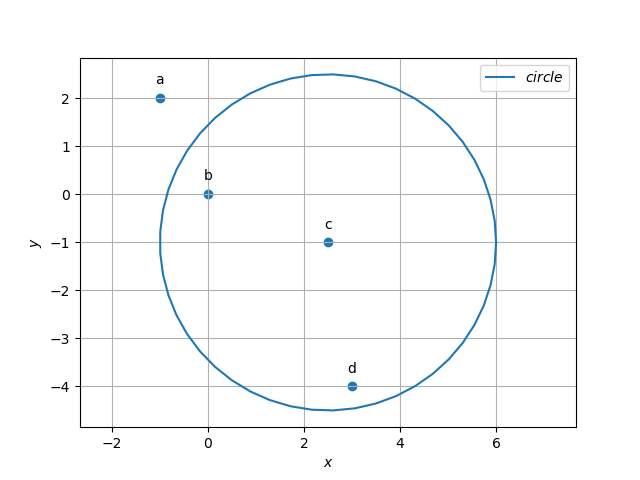
\includegraphics[width=\columnwidth]{./solutions/4/2/1/assign4}
\caption{Points a,b,d in the circle with center c}
\label{eq:solutions/4/2/1/Fig:1}
\end{figure}


